\documentclass[11pt,aspectratio=169]{beamer}

\usepackage{fontspec}
\usepackage{polyglossia}
\setdefaultlanguage{greek}
\setotherlanguage{english}
\setmainfont{Arial Unicode.ttf}[Path=/System/Library/Fonts/Supplemental/,Script=Greek]
\setsansfont{Arial Unicode.ttf}[Path=/System/Library/Fonts/Supplemental/,Script=Greek]
\setmonofont{Menlo}[Scale=0.86]
\newfontfamily\greekfont{Arial Unicode.ttf}[Path=/System/Library/Fonts/Supplemental/,Script=Greek]
\newfontfamily\greekfontsf{Arial Unicode.ttf}[Path=/System/Library/Fonts/Supplemental/,Script=Greek]
\newfontfamily\greekfonttt{Arial Unicode.ttf}[Path=/System/Library/Fonts/Supplemental/,Script=Greek,Scale=0.86]

\usepackage{graphicx}
\usepackage{booktabs}
\usepackage{tikz}

\graphicspath{{report/figures/}{figures/}}

% ---- Clean custom theme ----
\usetheme{default}
\useinnertheme{rectangles}
\setbeamertemplate{navigation symbols}{}
\definecolor{piraeus}{RGB}{17,58,108}
\definecolor{accent}{RGB}{0,150,160}
\definecolor{warm}{RGB}{214,108,28}
\definecolor{inkgray}{RGB}{60,66,74}
\definecolor{lightbg}{RGB}{244,247,250}

\setbeamercolor{structure}{fg=piraeus}
\setbeamercolor{frametitle}{fg=piraeus}
\setbeamercolor{normal text}{fg=inkgray}
\setbeamercolor{itemize item}{fg=accent}
\setbeamercolor{itemize subitem}{fg=warm}
\setbeamercolor{title}{fg=piraeus}
\setbeamercolor{author}{fg=inkgray}
\setbeamerfont{frametitle}{series=\bfseries,size=\large}
\setbeamerfont{title}{series=\bfseries}
\setbeamertemplate{itemize item}{\small\raise0.2ex\hbox{\textbullet}}
\setbeamertemplate{itemize subitem}{\scriptsize\raise0.2ex\hbox{--}}

% Frame title with accent rule
\setbeamertemplate{frametitle}{%
  \vskip0.6em%
  \begin{beamercolorbox}[wd=\paperwidth,leftskip=0.9em,rightskip=0.9em]{frametitle}%
    \usebeamerfont{frametitle}\insertframetitle%
  \end{beamercolorbox}%
  \vskip-0.3em%
  {\color{accent}\rule{\paperwidth}{1.2pt}}%
  \vskip0.2em%
}

% Footline
\setbeamertemplate{footline}{%
  \hbox{%
    \begin{beamercolorbox}[wd=.5\paperwidth,ht=2.2ex,dp=1ex,leftskip=0.9em]{}%
      \tiny\color{inkgray!80}Φαίδων Γραμματικόπουλος — mtn2505%
    \end{beamercolorbox}%
    \begin{beamercolorbox}[wd=.5\paperwidth,ht=2.2ex,dp=1ex,rightskip=0.9em]{}%
      \hfill\tiny\color{inkgray!80}\insertframenumber\,/\,\inserttotalframenumber%
    \end{beamercolorbox}%
  }%
  \vskip2pt%
}

\newcommand{\code}[1]{{\ttfamily\small #1}}
\newcommand{\num}[1]{{\bfseries\color{piraeus}#1}}

\begin{document}

% ---------- 1. TITLE ----------
{
\setbeamertemplate{footline}{}
\begin{frame}[plain]
  \vfill
  \begin{center}
    {\color{accent}\rule{0.55\paperwidth}{1.2pt}}\\[1.1em]
    {\usebeamerfont{title}\LARGE\color{piraeus}Υβριδικό Σύστημα Συστάσεων\\[0.25em]στο Amazon Reviews 2023}\\[0.7em]
    {\large\color{warm}Video Games case study}\\[1.2em]
    {\color{accent}\rule{0.55\paperwidth}{1.2pt}}\\[1.4em]
    {\large Φαίδων Γραμματικόπουλος \quad\textbar\quad \code{mtn2505}}\\[0.5em]
    {\small\color{inkgray!80}MSc in Artificial Intelligence\\University of Piraeus \& NCSR ``Demokritos''}\\[1.0em]
    {\small\color{piraeus}\code{github.com/Fgram-devAI/amazon-hybrid-recsys}}
  \end{center}
  \vfill
\end{frame}
}

% ---------- 2. PROBLEM DEFINITION ----------
\begin{frame}{Ορισμός προβλήματος}
  \begin{itemize}
    \item Στόχος: για χρήστη με γνωστό ιστορικό, προτείνουμε \alert{νέα} (μη ιδωμένα) αντικείμενα Amazon.
    \item \textbf{Content-based filtering}: ομοιότητα περιεχομένου — αδύναμο όταν τα metadata είναι φτωχά.
    \item \textbf{Collaborative filtering}: μοτίβα συμπεριφοράς χρηστών — ευάλωτο σε αραιότητα / cold-start.
    \item \textbf{Υβριδική προσέγγιση}: κάθε οικογένεια καλύπτει την αδυναμία της άλλης.
    \item Δύο όψεις του προβλήματος: \emph{rating prediction} (RMSE/MAE) και \emph{top-K recommendation} (P/R/F1).
  \end{itemize}
\end{frame}

% ---------- 3. DATASET CHOICE ----------
\begin{frame}{Επιλογή δεδομένων: Amazon Reviews 2023}
  \begin{itemize}
    \item \textbf{\code{Video\_Games}} — κύριο benchmark: επιβιώνει το αυστηρό 5-core, πυκνό αλλά διαχειρίσιμο τοπικά.
    \item \textbf{\code{Movies\_and\_TV}} — scale case: $\sim$7,4M αλληλεπιδράσεις· ελέγχει ότι το pipeline κλιμακώνεται.
    \item \textbf{\code{Digital\_Music}} — sparsity / cold-start case: το 5-core πρακτικά το αδειάζει.
  \end{itemize}
  \vskip0.4em
  \footnotesize
  \begin{center}
  \begin{tabular}{lrr}
    \toprule
    Dataset & Interactions & Users / Items \\
    \midrule
    \code{Video\_Games}  & 814.586   & 94.762 / 25.612 \\
    \code{Movies\_and\_TV} & 7.441.129 & 657.203 / 197.943 \\
    \code{Digital\_Music} & μικρός πυρήνας & --- (cold-start) \\
    \bottomrule
  \end{tabular}
  \end{center}
\end{frame}

% ---------- 4. PREPROCESSING ----------
\begin{frame}{Ροή προεπεξεργασίας (Pipeline / Funnel)}
  \begin{columns}[T]
    \begin{column}{0.5\textwidth}
      \begin{itemize}
        \item Αποδιπλοποίηση ζευγών \code{(user, item)} — κρατάμε το πιο πρόσφατο.
        \item \textbf{5-core filtering} ($k{=}2$ για \code{Digital\_Music}).
        \item Per-user \textbf{χρονολογικό} 80/20 split (seed 42).
        \item Χειρισμός missing metadata, ευθυγράμμιση στο \code{parent\_asin}.
        \item \alert{Κανόνας διαρροής}: features \& ακμές γράφου μόνο από το \emph{train}.
      \end{itemize}
    \end{column}
    \begin{column}{0.5\textwidth}
      \centering
      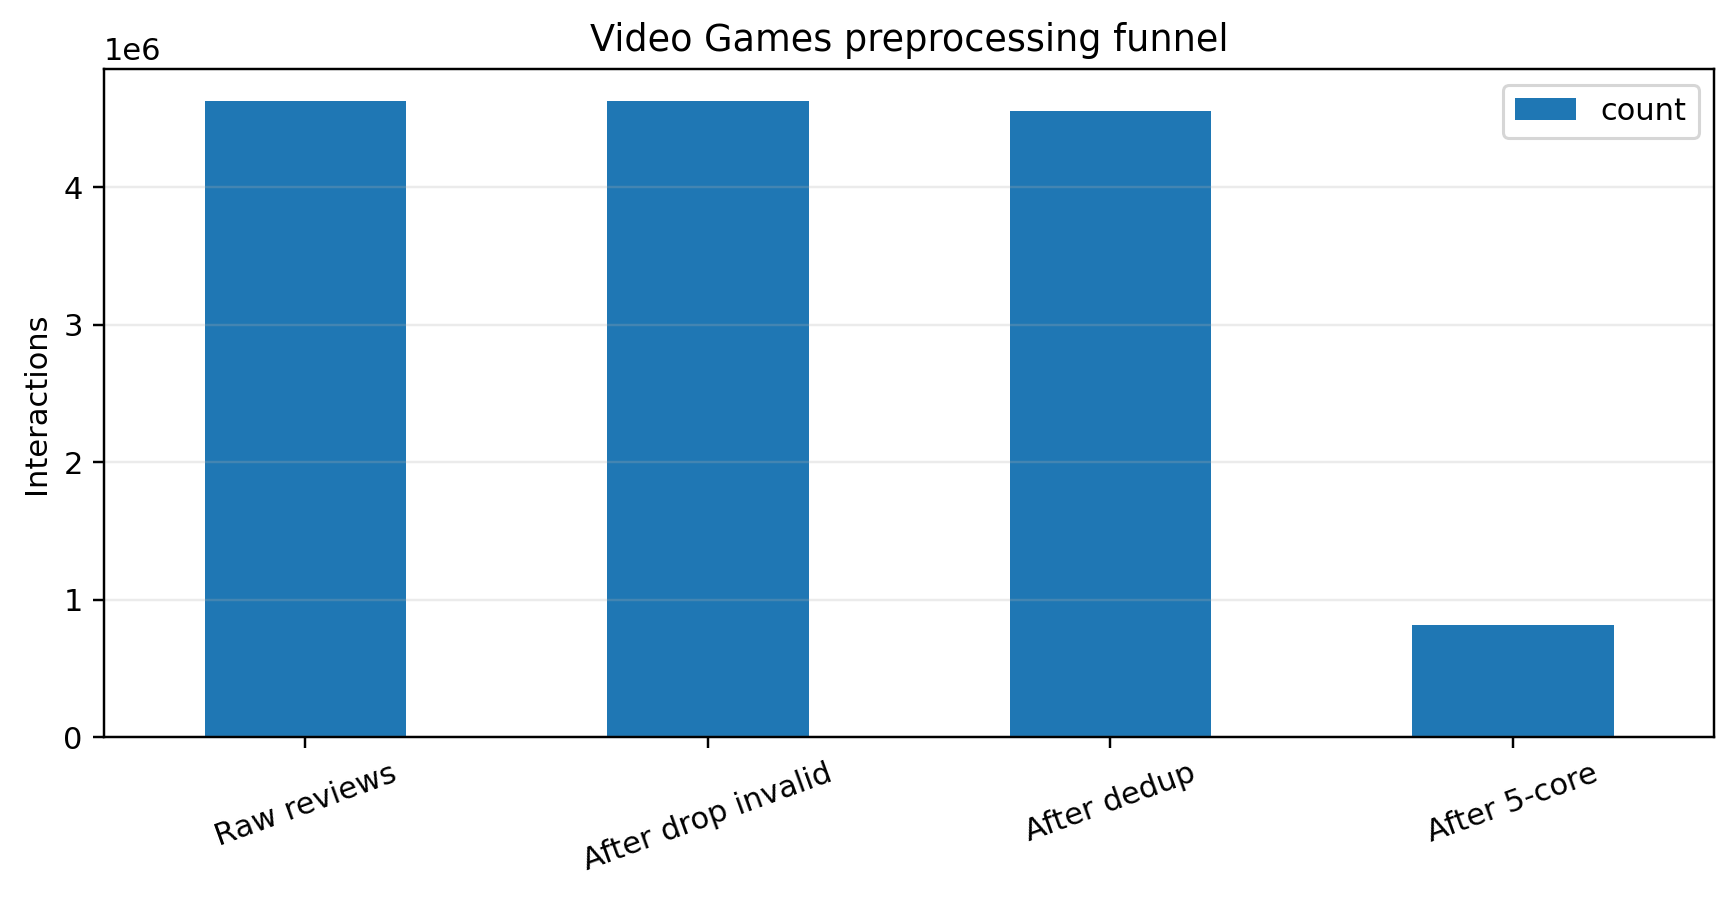
\includegraphics[width=\linewidth]{preprocessing_funnel.png}\\
      \tiny 4,62M → dedup 4,56M → 5-core \num{814.586}
    \end{column}
  \end{columns}
\end{frame}

% ---------- 5. DATASET CHARACTERISTICS ----------
\begin{frame}{Χαρακτηριστικά του dataset}
  \begin{columns}[T]
    \begin{column}{0.5\textwidth}
      \begin{itemize}
        \item Μετά το 5-core: \num{94.762} χρήστες, \num{25.612} items, \num{814.586} αλληλεπιδράσεις.
        \item Sparsity $\approx$ \num{0.9997} (πολύ αραιό ακόμη και μετά το core).
        \item Κλίση προς θετικά: \num{80,4\%} των ratings $\geq 4$ (κορυφή στα 5 αστέρια).
        \item Χωρίς resampling: κρατάμε τη φυσική κατανομή του implicit feedback.
        \item Γι' αυτό το χαμηλό raw P@10 ερμηνεύεται \emph{πάντα} έναντι popularity / oracle.
      \end{itemize}
    \end{column}
    \begin{column}{0.5\textwidth}
      \centering
      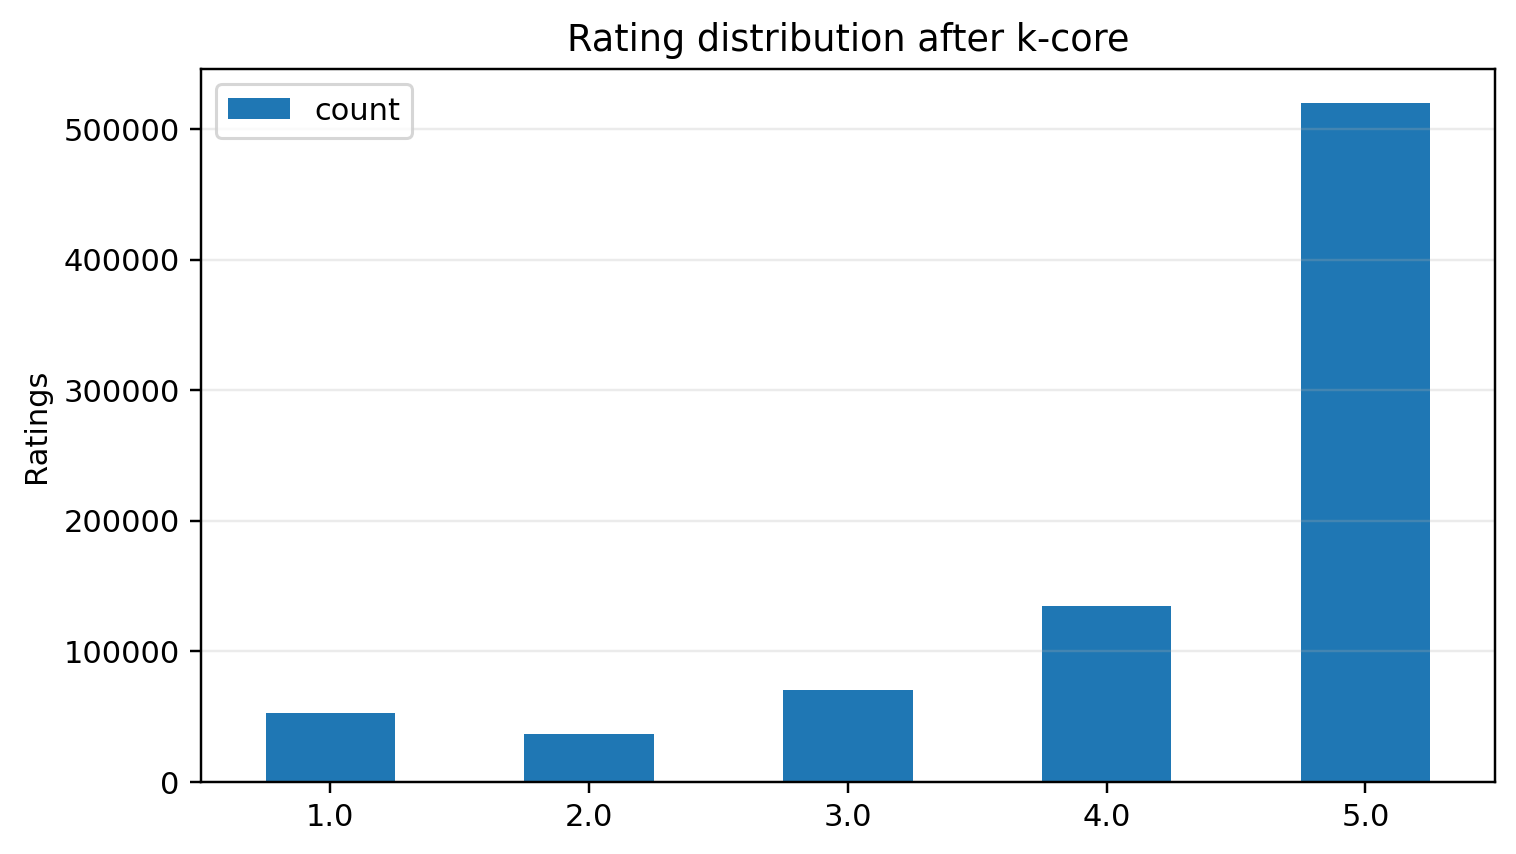
\includegraphics[width=\linewidth]{rating_distribution.png}\\
      \tiny Κατανομή ratings μετά το 5-core
    \end{column}
  \end{columns}
\end{frame}

% ---------- 6. EVALUATION PROTOCOL ----------
\begin{frame}{Πρωτόκολλο αξιολόγησης}
  \begin{itemize}
    \item \textbf{Rating prediction}: RMSE, MAE στο held-out test split.
    \item \textbf{Ranking}: Precision@10, Recall@10, F1@10 (σχετικό = rating $\geq 4$).
    \item \textbf{Audit μετρικές}: HitRate@10, NDCG@10.
    \item \textbf{Sampled-candidate}: ανά χρήστη, held-out positives $+\,N{=}100$ τυχαία negatives (seed 42, ίδια για όλα τα μοντέλα).
    \item \textbf{Oracle ceiling}: διάμεσος $\approx 1$ σχετικό item/χρήστη $\Rightarrow$ \num{$P^\star@10=0{,}1552$}, \num{$F1^\star@10=0{,}2551$}.
  \end{itemize}
  \vskip0.3em
  \footnotesize\color{inkgray!85} Sampled, όχι full-catalog: τα νούμερα δεν συγκρίνονται άμεσα με άλλες εργασίες.
\end{frame}

% ---------- 7. CLASSIC CF BASELINES ----------
\begin{frame}{Κλασικά Collaborative Filtering baselines}
  \begin{columns}[T]
    \begin{column}{0.52\textwidth}
      \begin{itemize}
        \item \textbf{Item-KNN} (\code{KNNWithMeans}, item-based): ομοιότητα items από κοινές αξιολογήσεις.
        \item \textbf{SVD / matrix factorization}: λανθάνοντα διανύσματα χρηστών \& items $+$ bias όροι.
        \item Σήμα μόνο από τον πίνακα ratings — όχι κείμενο/metadata.
        \item \alert{SVD}: ισχυρότερο σε RMSE (\num{1,1337}) αλλά αδύναμο top-K (F1@10 \num{0,0543}).
      \end{itemize}
      \footnotesize\color{inkgray!85}Διαφορετικό objective $\Rightarrow$ διαφορετικός νικητής.
    \end{column}
    \begin{column}{0.48\textwidth}
      \centering
      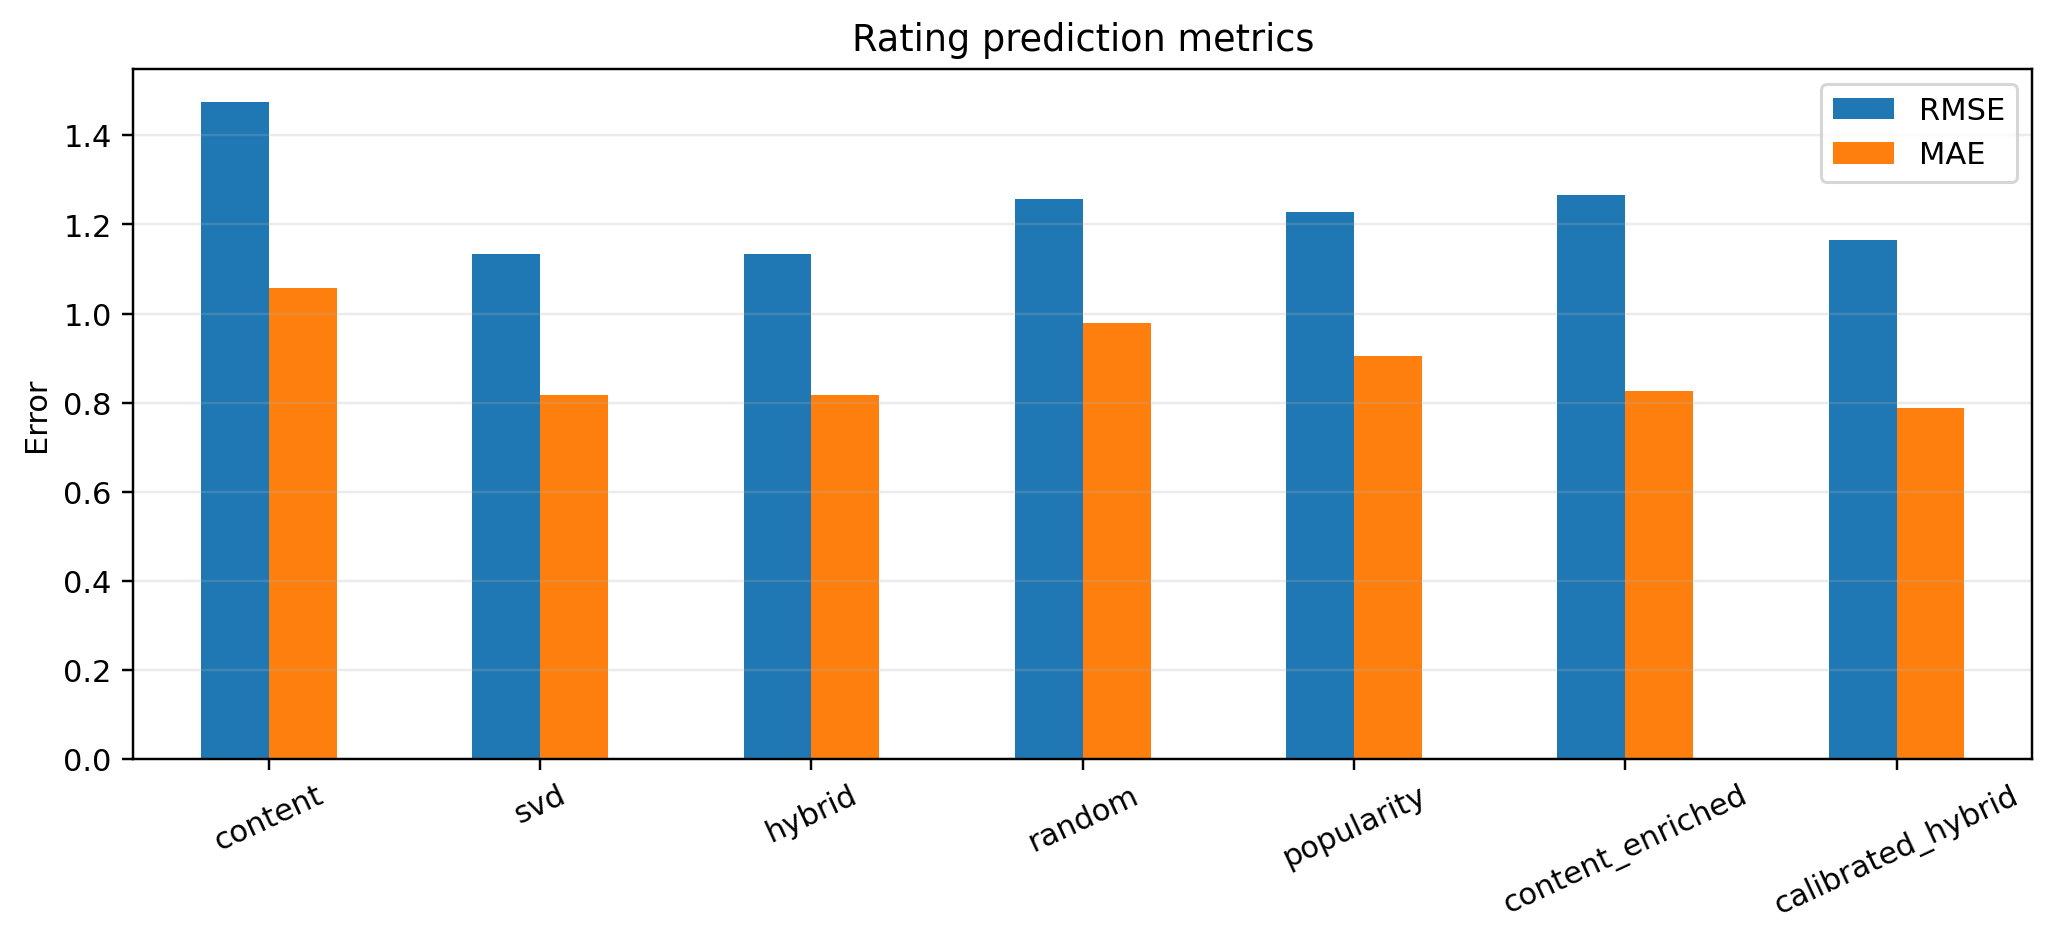
\includegraphics[width=\linewidth]{model_error_metrics.png}\\
      \tiny RMSE \& MAE — βασικά \& εμπλουτισμένα μοντέλα
    \end{column}
  \end{columns}
\end{frame}

% ---------- 8. CONTENT-BASED ----------
\begin{frame}{Content-based filtering}
  \begin{itemize}
    \item Προφίλ item από \code{title + description + categories} $+$ αριθμητικά metadata (\code{price}, \code{avg\_rating}, \code{rating\_number}).
    \item Transformer embeddings: \code{granite-embedding-97m-multilingual-r2}, $\ell_2$-normalized.
    \item Πρόβλεψη: σταθμισμένος μέσος αξιολογήσεων ιστορικού με βάρη \textbf{cosine similarity}.
    \item Χωρίς κλασική NLP προεπεξεργασία (stemming/lemmatization): τα embeddings αξιοποιούν σειρά \& συμφραζόμενα.
    \item Plain content: F1@10 \num{0,0675} — κάτω από το popularity (\num{0,1284}): η σημασιολογία βοηθά αλλά δεν αρκεί.
  \end{itemize}
\end{frame}

% ---------- 9. HYBRID & ENRICHED ----------
\begin{frame}{Υβριδικά \& εμπλουτισμένα content μοντέλα}
  \begin{itemize}
    \item \textbf{Weighted hybrid}: $\hat r = \alpha\cdot\text{CF} + (1-\alpha)\cdot\text{content}$ — με RMSE-tuned $\alpha\approx 1$ καταρρέει στο SVD.
    \item \textbf{Calibrated hybrid}: z-score recentering πριν τη μίξη· εξισορροπεί RMSE (\num{1,1737}), MAE (\num{0,7679}) \& F1@10 (\num{0,1003}).
    \item \textbf{\code{content\_enriched}}: φιλτραρισμένες κατηγορίες, αριθμητικά metadata, \emph{train-only} sentiment (DistilBERT-SST2) \& user-generosity offset.
    \item Sentiment: F1@10 \num{0,1047} $\rightarrow$ \num{0,1250}, αλλά MAE \num{0,7917} $\rightarrow$ \num{0,8258} — \alert{προαιρετικό} ranking feature.
  \end{itemize}
\end{frame}

% ---------- 10. GRAPH RECOMMENDERS ----------
\begin{frame}{Graph recommenders}
  \begin{columns}[T]
    \begin{column}{0.52\textwidth}
      \begin{itemize}
        \item \textbf{Train-only} διμερικός γράφος user--item (test ακμές ποτέ σε message passing).
        \item \textbf{LightGCN}: καθαρά collaborative ranker, BPR — \alert{ισχυρότερος} (F1@10 \num{0,1492}, $\approx 58{,}5\%$ του oracle).
        \item \textbf{GraphSAGE-MSE}: graph $+$ node features, rating regressor (RMSE \num{1,1613}).
        \item \textbf{GraphSAGE-BPR}: ranking-oriented· βελτιώνει το ranking αλλά υστερεί του LightGCN.
      \end{itemize}
    \end{column}
    \begin{column}{0.48\textwidth}
      \centering
      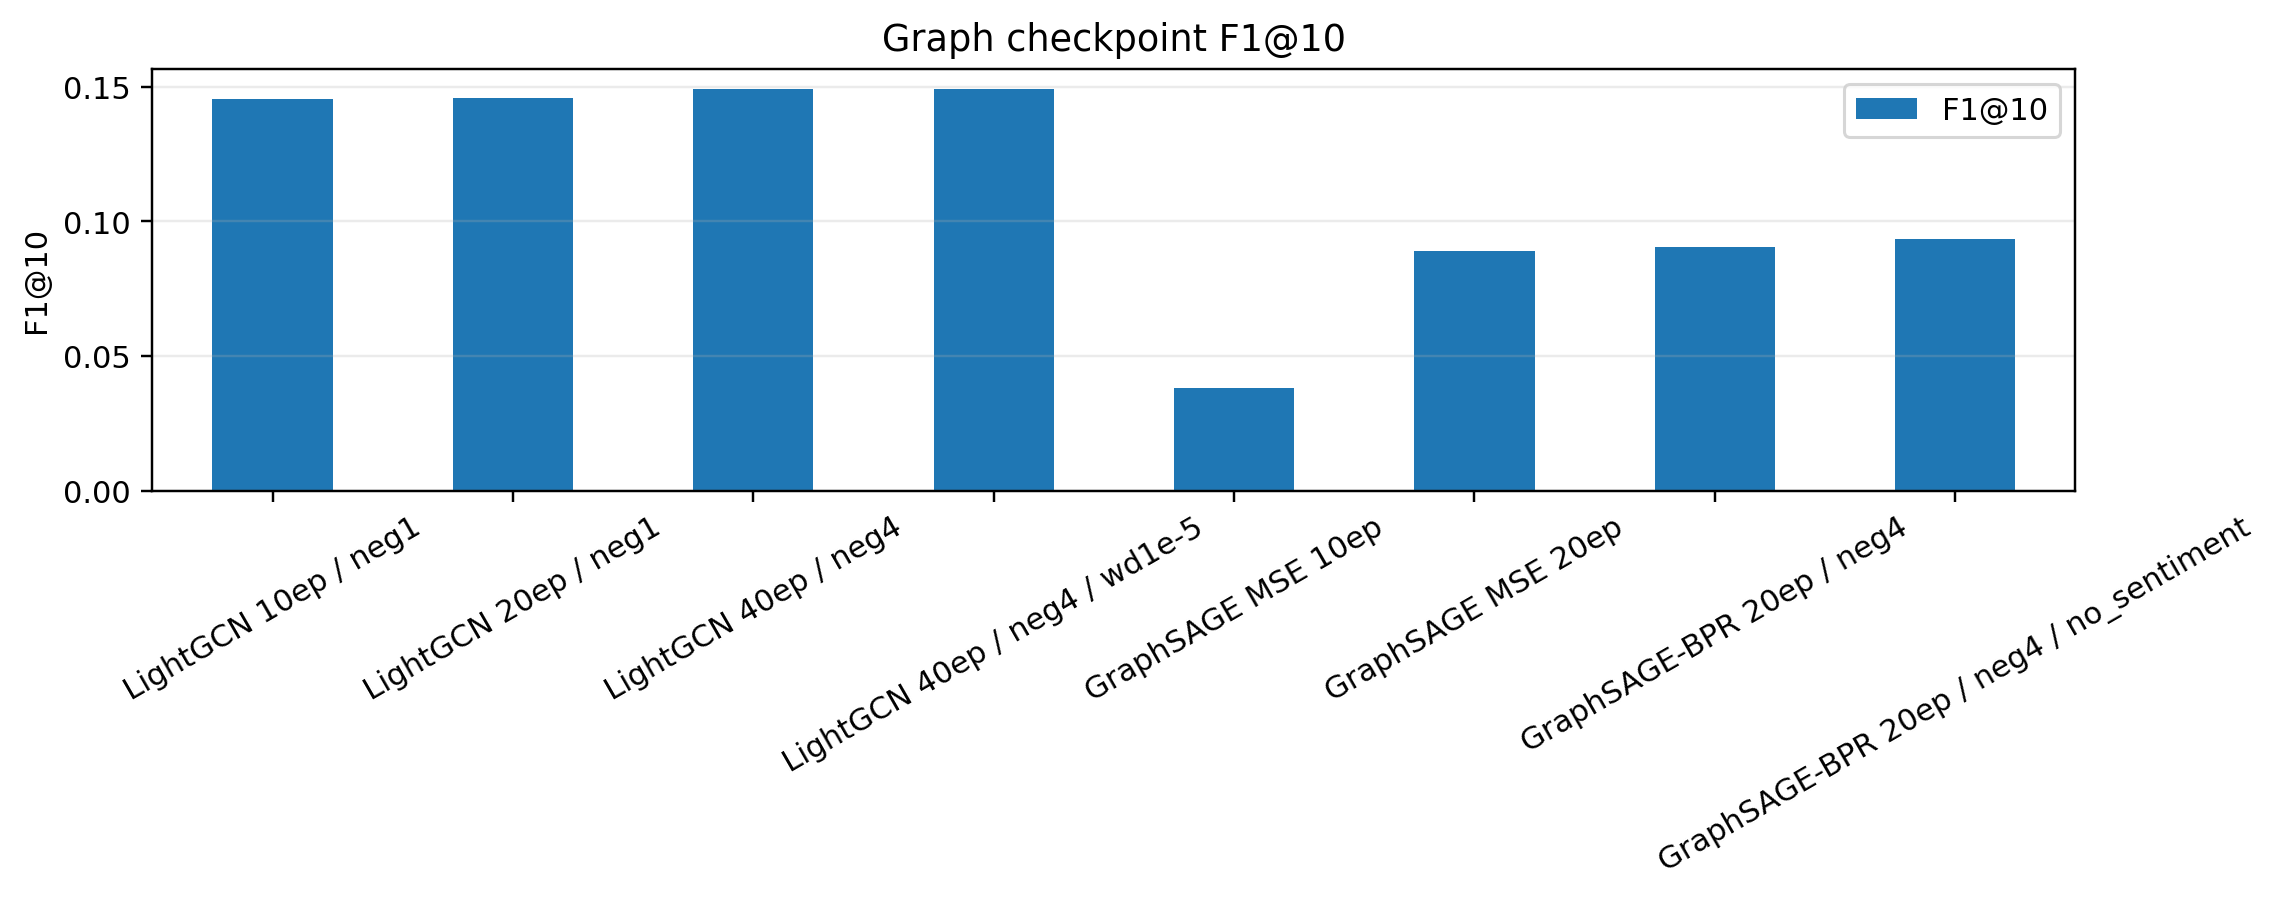
\includegraphics[width=\linewidth]{graph_checkpoint_f1.png}\\
      \tiny F1@10 graph checkpoints (ίδιο sampled πρωτόκολλο)
    \end{column}
  \end{columns}
\end{frame}

% ---------- 11. GRAPH EDA / COMMUNITIES ----------
\begin{frame}{Graph EDA / ανάλυση κοινοτήτων}
  \begin{itemize}
    \item Item--item \emph{co-rating projection}: ακμή όταν δύο items αξιολογούνται θετικά από κοινούς χρήστες.
    \item Κοινότητες με Louvain, Leiden, Spectral, Girvan--Newman· ευθυγράμμιση με κατηγορίες (purity, NMI).
    \item \alert{Ερμηνευσιμότητα}, όχι training signal του recommender.
  \end{itemize}
  \vskip0.2em
  \begin{columns}[c]
    \begin{column}{0.5\textwidth}\centering
      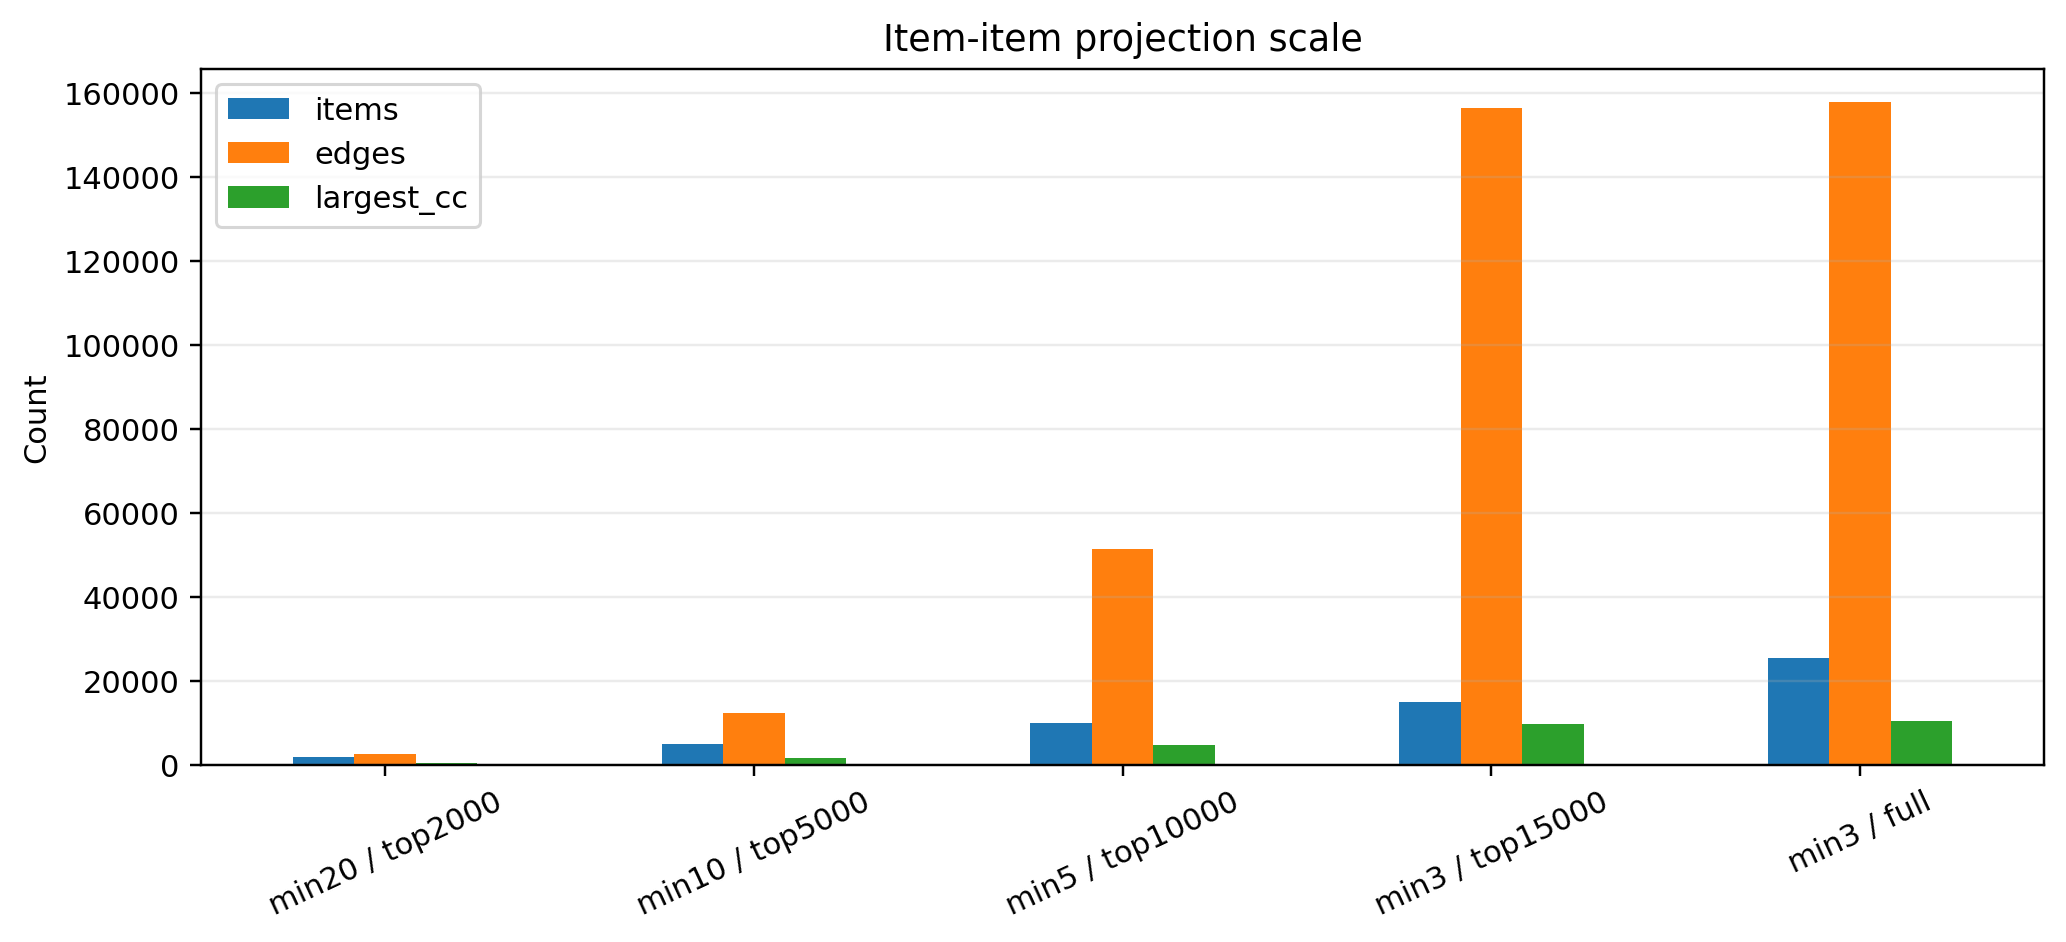
\includegraphics[width=0.96\linewidth]{graph_projection_scale.png}\\ \tiny Κλίμακα projection ανά threshold
    \end{column}
    \begin{column}{0.5\textwidth}\centering
      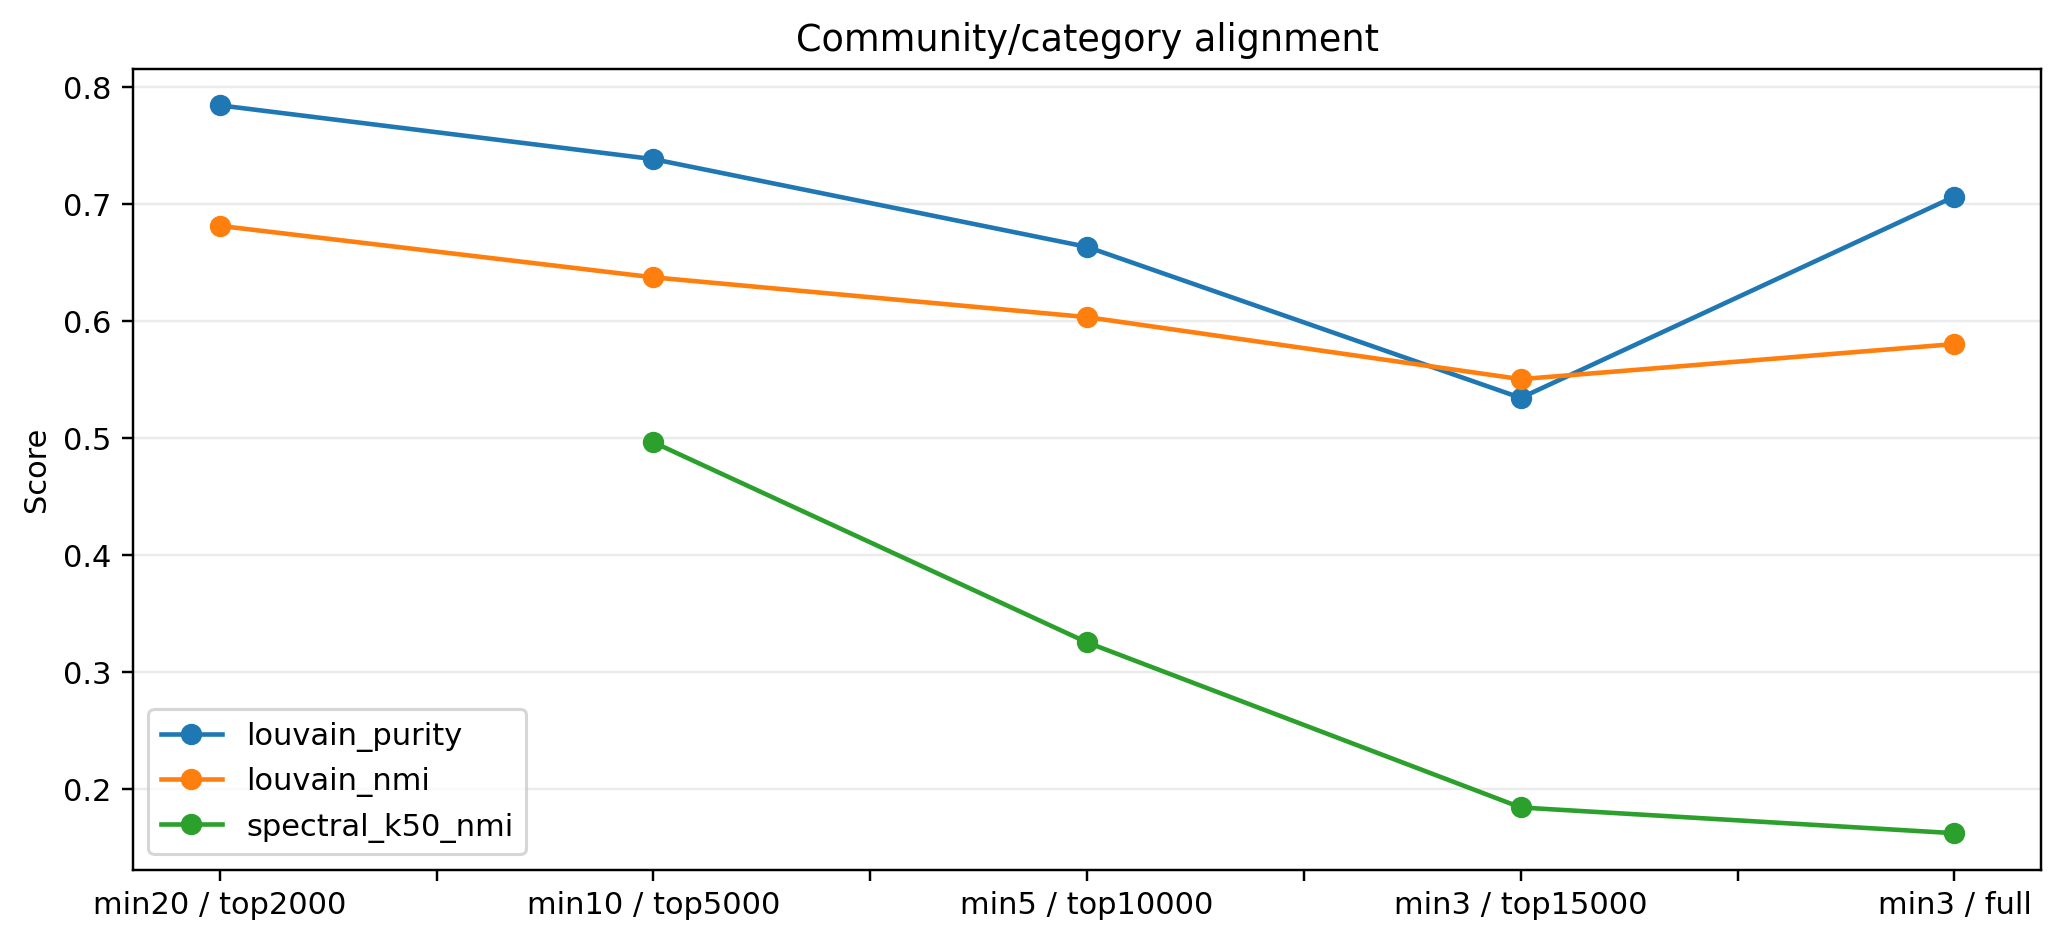
\includegraphics[width=0.96\linewidth]{community_alignment.png}\\ \tiny Ευθυγράμμιση κοινοτήτων--κατηγοριών
    \end{column}
  \end{columns}
\end{frame}

% ---------- 12. MAIN RESULTS ----------
\begin{frame}{Κύρια αποτελέσματα (\code{video\_games})}
  \begin{columns}[T]
    \begin{column}{0.5\textwidth}
      \begin{itemize}
        \item \textbf{SVD} κερδίζει το classic RMSE (\num{1,1337}).
        \item \textbf{Popularity}: ισχυρό sampled-ranking baseline (F1@10 \num{0,1284}).
        \item \code{content\_enriched} πλησιάζει το popularity (F1@10 \num{0,1250}).
        \item \textbf{LightGCN}: ισχυρότερος ranker (F1@10 \num{0,1492}).
        \item GraphSAGE-MSE: καλύτερη rating regression· BPR βελτιώνει ranking αλλά $<$ LightGCN.
      \end{itemize}
    \end{column}
    \begin{column}{0.5\textwidth}
      \centering
      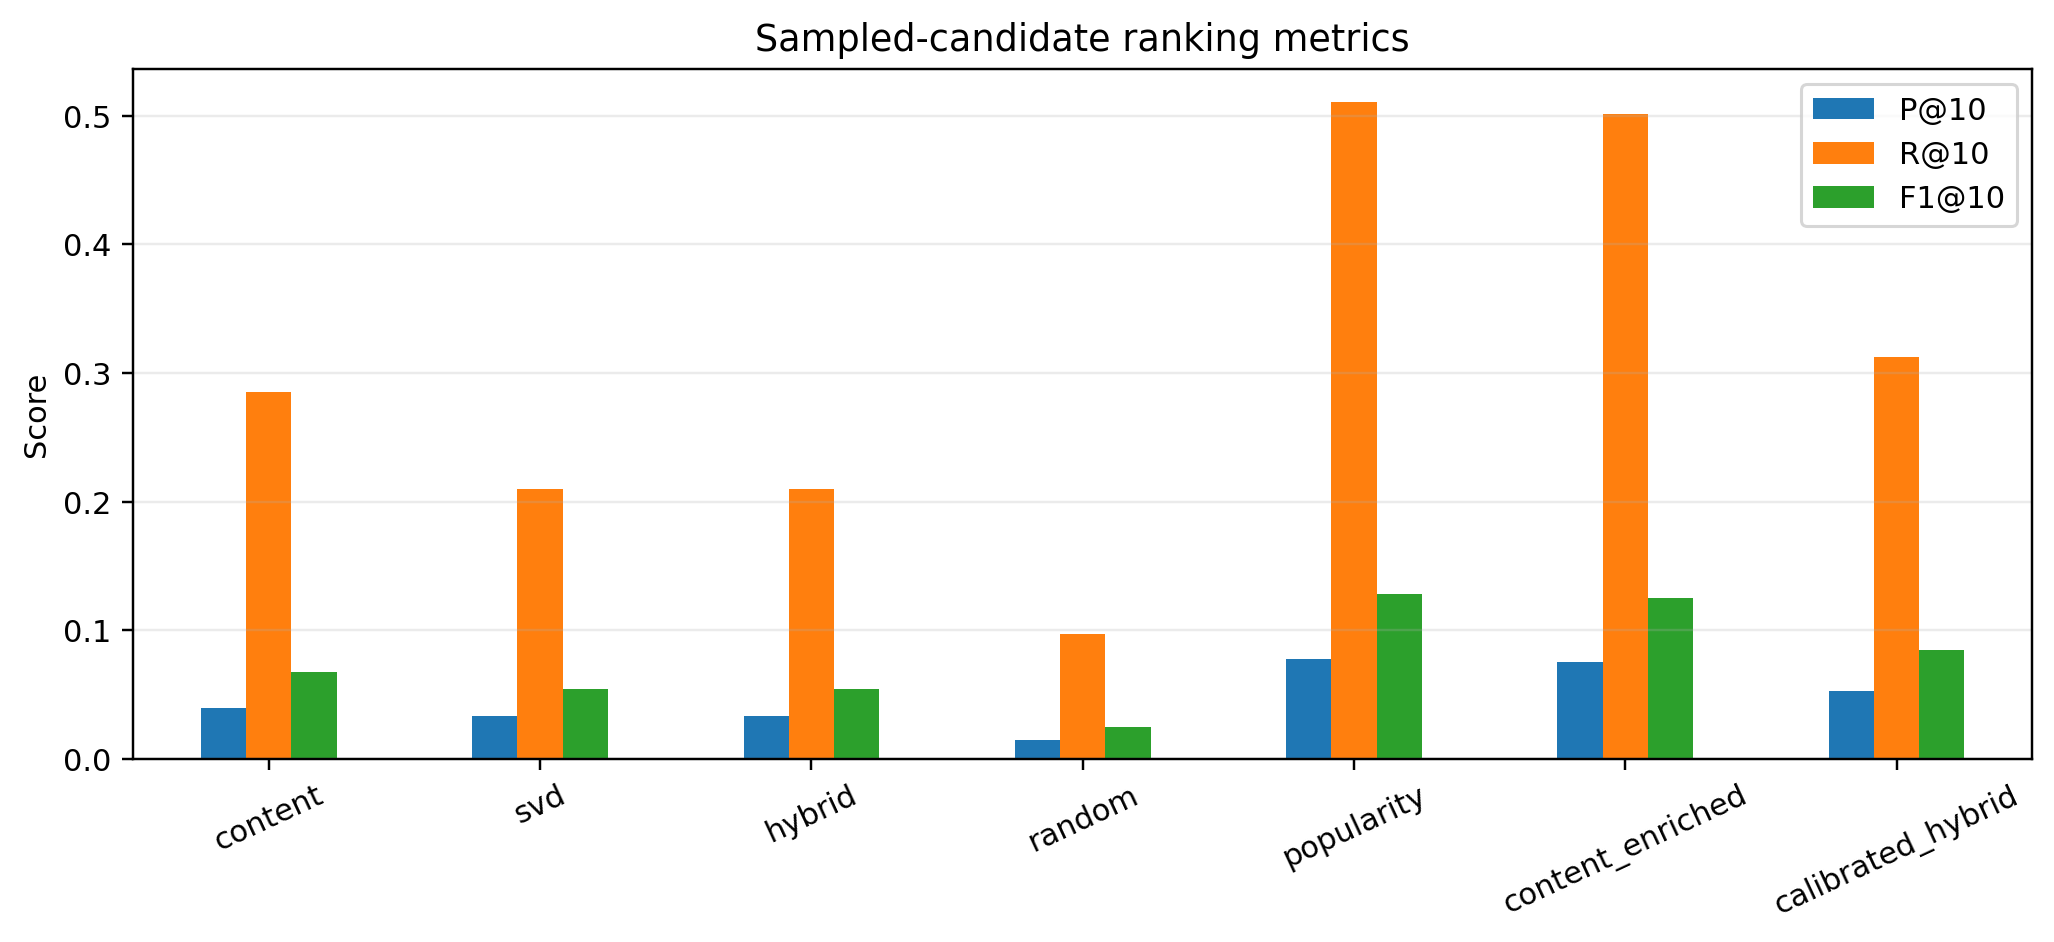
\includegraphics[width=\linewidth]{model_ranking_metrics.png}\\
      \tiny Sampled-candidate P@10 / R@10 / F1@10
    \end{column}
  \end{columns}
\end{frame}

% ---------- 13. APPLICATION LAYER ----------
\begin{frame}{Επίπεδο εφαρμογής — Streamlit}
  \begin{itemize}
    \item Διαδραστικό dashboard πάνω από τοπικά ή demo artifacts.
    \item Καρτέλες: Overview, Model Comparison, Graph Models + Ablations, Graph EDA, Item Explorer, Recommendations.
    \item Δεν υπολογίζει ξανά embeddings ή graph checkpoints· για διαδραστική χρήση μπορεί να κάνει ελαφρύ τοπικό fit σε SVD/KNN.
    \item \textbf{Recommendations}: popularity, SVD, KNN (cosine/pearson/msd), content enriched, calibrated hybrid, LightGCN και LLM hybrid (profile/query).
    \item \alert{Ποιοτική επιθεώρηση} — δεν αντικαθιστά τις μετρικές RMSE/MAE/P/R/F1.
  \end{itemize}
\end{frame}

% ---------- 14. RETRIEVAL / EXPLANATION ----------
\begin{frame}{Υποδομή ανάκτησης \& εξήγησης}
  \begin{itemize}
    \item \textbf{Milvus Lite}: vector search πάνω στα item embeddings (semantic neighbors).
    \item \textbf{Neo4j}: \emph{train-only} γράφος user--item--category ως τεκμήρια εξήγησης.
    \item \textbf{LLM layer} (Groq, OpenAI-compatible): φυσικογλωσσική εξήγηση πάνω σε structured evidence.
    \item \alert{Σημαντικό}: το LLM \emph{εξηγεί} ντετερμινιστικές συστάσεις — δεν αναδιατάσσει top-K, δεν αντικαθιστά τις αξιολογούμενες μετρικές.
  \end{itemize}
  \vskip0.3em
  \footnotesize\color{inkgray!85} Προαιρετικό επίπεδο· συμβατό με τον κανόνα διαρροής (test ratings δεν εισάγονται).
\end{frame}

% ---------- 15. CONCLUSIONS ----------
\begin{frame}{Συμπεράσματα \& αποθετήριο}
  \begin{itemize}
    \item Κανένα μοντέλο δεν κερδίζει σε όλα — ο \textbf{στόχος} καθορίζει τον νικητή.
    \item \emph{Rating prediction}: SVD \quad\textbar\quad \emph{Top-K ranking}: LightGCN.
    \item Το collaborative graph signal είναι το ισχυρότερο για ranking.
    \item Content \& review-feedback βοηθούν, αλλά δεν αντικαθιστούν το collaborative σήμα.
    \item \textbf{Μελλοντικά}: full-catalog evaluation, sequence-aware (SASRec/BERT4Rec), ισχυρότερα GNN, καλύτερες LLM εξηγήσεις.
  \end{itemize}
  \vskip0.6em
  \begin{center}
    {\color{accent}\rule{0.5\paperwidth}{1pt}}\\[0.5em]
    {\small\color{piraeus}\code{github.com/Fgram-devAI/amazon-hybrid-recsys}}
  \end{center}
\end{frame}

\end{document}
